% Winners and losers against actuated lights, trip by trip (analyze/winners_losers_analysis.py).
\begin{figure}[H]
    \centering
    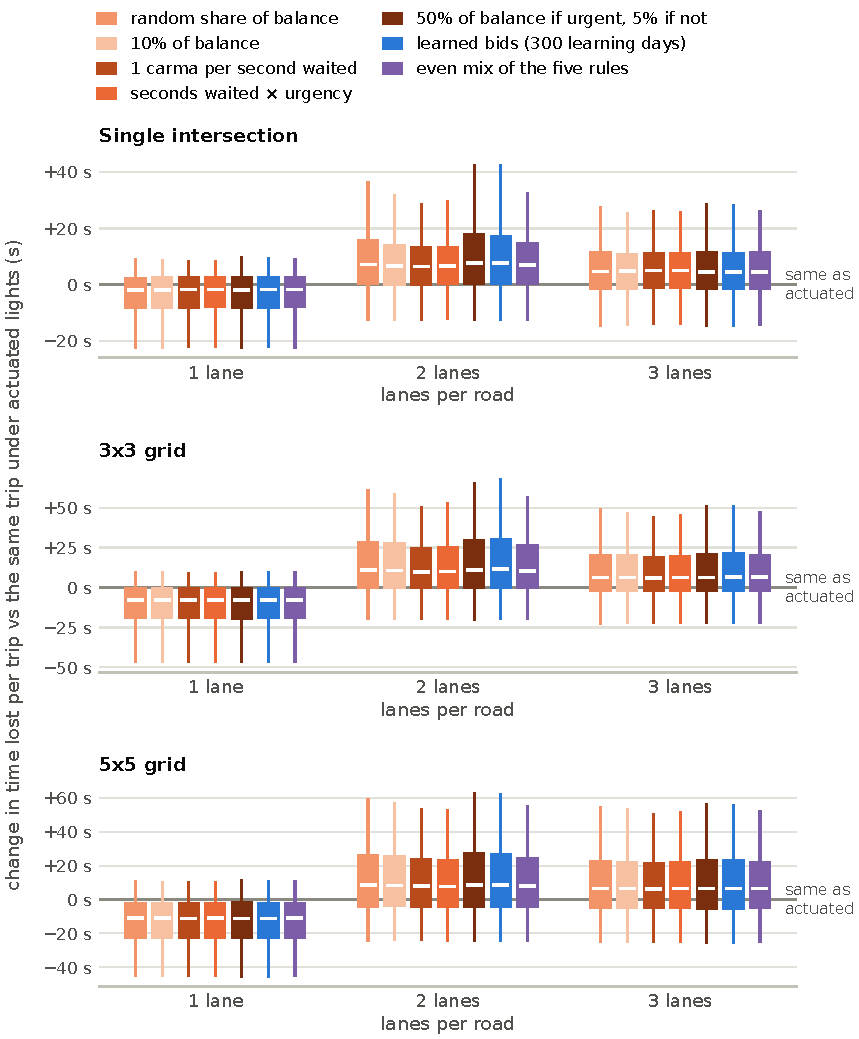
\includegraphics[width=\linewidth]{winners_losers_spread.pdf}
    \caption{Who wins and who loses when every driver uses the same rule: each trip of the
    evaluation week is paired with the very same trip under actuated lights, and the change in
    its time lost is spread over the trips. Box: the middle half of trips (25th to 75th
    percentile); line: 5th to 95th percentile; white tick: median. Below 0 the trip is faster than
    under actuated lights. Reference setting; fixed rules after 7 warm-up days, learned bids after
    300 learning days; percentiles are means of 10 seeds; each panel has its own scale.}
    \label{fig:winners_losers_spread}
\end{figure}

\begin{figure}[H]
    \centering
    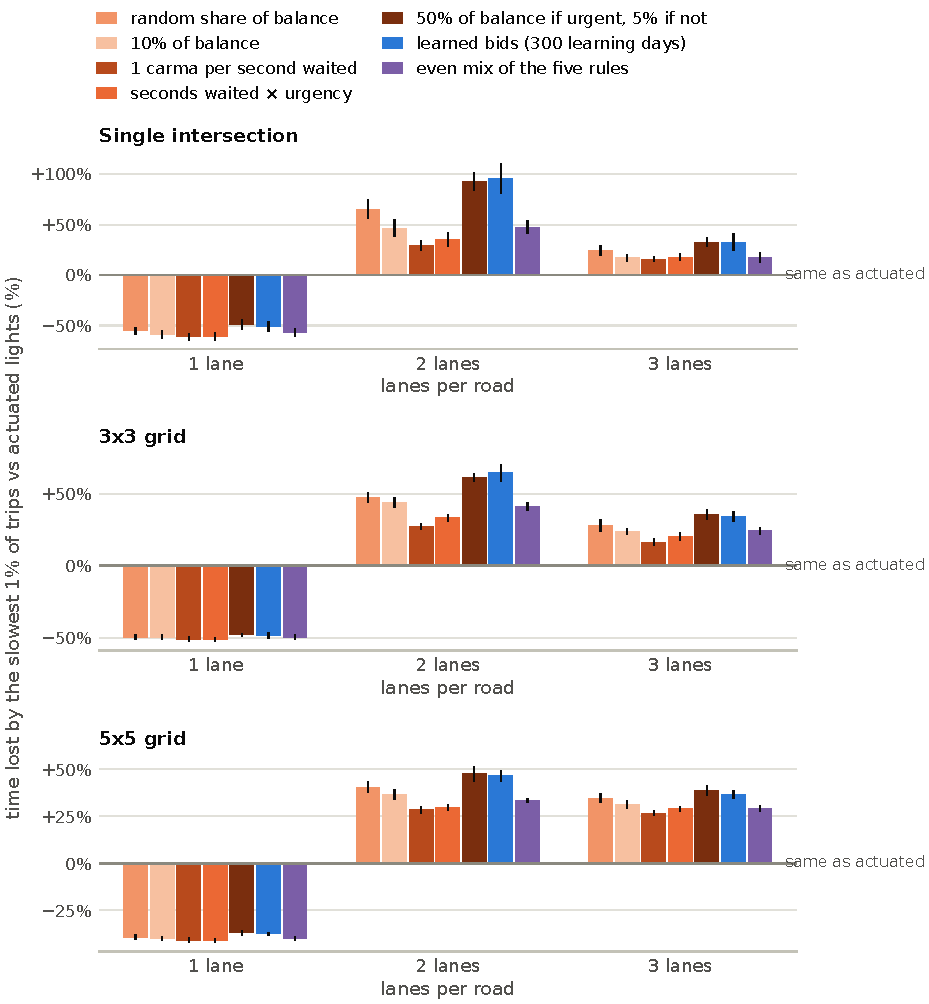
\includegraphics[width=\linewidth]{winners_losers_tail.pdf}
    \caption{The worst-off trips: time lost by the slowest 1\% of trips (99th percentile),
    compared with the slowest 1\% under actuated lights on the same trips. Settings as in
    Figure~\ref{fig:winners_losers_spread}; bars are means of 10 seeds, whiskers 95\%
    intervals; each panel has its own scale.}
    \label{fig:winners_losers_tail}
\end{figure}
